%package list
\documentclass{article}
\usepackage[top=3cm, bottom=3cm, outer=3cm, inner=3cm]{geometry}
\usepackage{multicol}
\usepackage{graphicx}
\usepackage{url}
%\usepackage{cite}
\usepackage{hyperref}
\usepackage{array}
%\usepackage{multicol}
\newcolumntype{x}[1]{>{\centering\arraybackslash\hspace{0pt}}p{#1}}
\usepackage{natbib}
\usepackage{pdfpages}
\usepackage{multirow}
\usepackage[normalem]{ulem}
\useunder{\uline}{\ul}{}
\usepackage{svg}
\usepackage{xcolor}
\usepackage{listings}
\lstdefinestyle{ascii-tree}{
    literate={├}{|}1 {─}{--}1 {└}{+}1 
  }
\lstset{basicstyle=\ttfamily,
  showstringspaces=false,
  commentstyle=\color{red},
  keywordstyle=\color{blue}
}
%\usepackage{booktabs}
\usepackage{caption}
\usepackage{subcaption}
\usepackage{float}
\usepackage{array}

\newcolumntype{M}[1]{>{\centering\arraybackslash}m{#1}}
\newcolumntype{N}{@{}m{0pt}@{}}


%%%%%%%%%%%%%%%%%%%%%%%%%%%%%%%%%%%%%%%%%%%%%%%%%%%%%%%%%%%%%%%%%%%%%%%%%%%%
%%%%%%%%%%%%%%%%%%%%%%%%%%%%%%%%%%%%%%%%%%%%%%%%%%%%%%%%%%%%%%%%%%%%%%%%%%%%
\newcommand{\itemEmail}{phidalgo@unsa.edu.pe}
\newcommand{\itemStudent}{Paulo Andre hidalgo Chinchay}
\newcommand{\itemCourse}{Programación web 2}
\newcommand{\itemCourseCode}{20223011}
\newcommand{\itemSemester}{III}
\newcommand{\itemUniversity}{Universidad Nacional de San Agustín de Arequipa}
\newcommand{\itemFaculty}{Facultad de Ingeniería de Producción y Servicios}
\newcommand{\itemDepartment}{Departamento Académico de Ingeniería de Sistemas e Informática}
\newcommand{\itemSchool}{Escuela Profesional de Ingeniería de Sistemas}
\newcommand{\itemAcademic}{2023 - A}
\newcommand{\itemInput}{Del 2 Junio 2023}
\newcommand{\itemOutput}{Al 5 Junio 2023}
\newcommand{\itemPracticeNumber}{01}
\newcommand{\itemTheme}{JavaScript}
%%%%%%%%%%%%%%%%%%%%%%%%%%%%%%%%%%%%%%%%%%%%%%%%%%%%%%%%%%%%%%%%%%%%%%%%%%%%
%%%%%%%%%%%%%%%%%%%%%%%%%%%%%%%%%%%%%%%%%%%%%%%%%%%%%%%%%%%%%%%%%%%%%%%%%%%%

\usepackage[english,spanish]{babel}
\usepackage[utf8]{inputenc}
\AtBeginDocument{\selectlanguage{spanish}}
\renewcommand{\figurename}{Figura}
\renewcommand{\refname}{Referencias}
\renewcommand{\tablename}{Tabla} %esto no funciona cuando se usa babel
\AtBeginDocument{%
	\renewcommand\tablename{Tabla}
}

\usepackage{fancyhdr}
\pagestyle{fancy}
\fancyhf{}
\setlength{\headheight}{30pt}
\renewcommand{\headrulewidth}{1pt}
\renewcommand{\footrulewidth}{1pt}
\fancyhead[L]{\raisebox{-0.2\height}{
\includegraphics[width=3cm]{img/logo_episunsa.png}}}
\fancyhead[C]{\fontsize{7}{7}\selectfont	\itemUniversity \\ \itemFaculty \\ \itemDepartment \\ \itemSchool \\ \textbf{\itemCourse}}
\fancyhead[R]{\raisebox{-0.2\height}{
\includegraphics[width=1.2cm]{img/logo_abet}}}
\fancyfoot[L]{Estudiante Paulo Hidalgo Chinchay}
\fancyfoot[C]{\itemCourse}
\fancyfoot[R]{Página \thepage}

% para el codigo fuente
\usepackage{listings}
\usepackage{color, colortbl}
\definecolor{dkgreen}{rgb}{0,0.6,0}
\definecolor{gray}{rgb}{0.5,0.5,0.5}
\definecolor{mauve}{rgb}{0.58,0,0.82}
\definecolor{codebackground}{rgb}{0.95, 0.95, 0.92}
\definecolor{tablebackground}{rgb}{0.8, 0, 0}

\lstset{frame=tb,
	language=bash,
	aboveskip=3mm,
	belowskip=3mm,
	showstringspaces=false,
	columns=flexible,
	basicstyle={\small\ttfamily},
	numbers=none,
	numberstyle=\tiny\color{gray},
	keywordstyle=\color{blue},
	commentstyle=\color{dkgreen},
	stringstyle=\color{mauve},
	breaklines=true,
	breakatwhitespace=true,
	tabsize=3,
	backgroundcolor= \color{codebackground},
}

\begin{document}
	
	\vspace*{10px}
	
	\begin{center}	
		\fontsize{17}{17} \textbf{ Informe de Laboratorio \itemPracticeNumber}
	\end{center}
	\centerline{\textbf{\Large Tema: \itemTheme}}
	%\vspace*{0.5cm}	

	\begin{flushright}
		\begin{tabular}{|M{2.5cm}|N|}
			\hline 
			\rowcolor{tablebackground}
			\color{white} \textbf{Nota}  \\
			\hline 
			     \\[30pt]
			\hline 			
		\end{tabular}
	\end{flushright}	

	\begin{table}[H]
		\begin{tabular}{|x{4.7cm}|x{4.8cm}|x{4.8cm}|}
			\hline 
			\rowcolor{tablebackground}
			\color{white} \textbf{Estudiante} & \color{white}\textbf{Escuela}  & \color{white}\textbf{Asignatura}   \\
			\hline 
			{\itemStudent \par \itemEmail} & \itemSchool & {\itemCourse \par Semestre: \itemSemester \par Código: \itemCourseCode}     \\
			\hline 			
		\end{tabular}
	\end{table}		
	
	\begin{table}[H]
		\begin{tabular}{|x{4.7cm}|x{4.8cm}|x{4.8cm}|}
			\hline 
			\rowcolor{tablebackground}
			\color{white}\textbf{Laboratorio} & \color{white}\textbf{Tema}  & \color{white}\textbf{Duración}   \\
			\hline 
			\itemPracticeNumber & \itemTheme & 04 horas   \\
			\hline 
		\end{tabular}
	\end{table}
	
	\begin{table}[H]
		\begin{tabular}{|x{4.7cm}|x{4.8cm}|x{4.8cm}|}
			\hline 
			\rowcolor{tablebackground}
			\color{white}\textbf{Semestre académico} & \color{white}\textbf{Fecha de inicio}  & \color{white}\textbf{Fecha de entrega}   \\
			\hline 
			\itemAcademic & \itemInput &  \itemOutput  \\
			\hline 
		\end{tabular}
	\end{table}
	
	\section{Tarea}
	\begin{itemize}		
		\item Utilizando JavaScript, genere un teclado aleatorio para Banca por Internet.
		Funcionalidad: Los números presionados generan una clave.		
		\item Utilizando JavaScript, genere una calculadora como la siguiente imagen. 
		\begin{figure}[H]
			\centering
			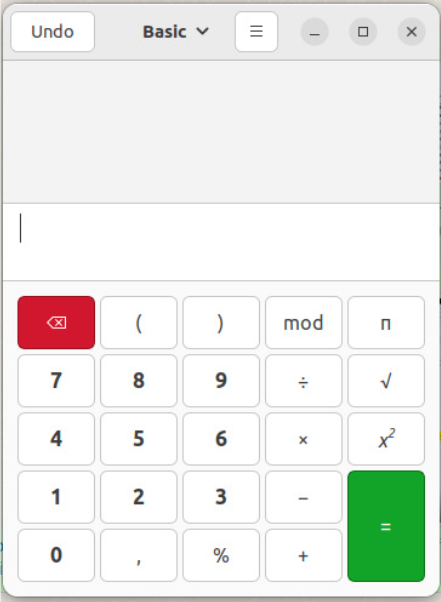
\includegraphics[width=0.3\textwidth,keepaspectratio]{img/calc.png}
		\end{figure}
		Con memoria y botones para recorrer la pila.
		Agregue 3 botones:
		M1: memoria
		M2: memoria
		ANS
	\end{itemize}
		
	\section{Equipos, materiales y temas utilizados}
	\begin{itemize}
		\item Sistema Operativo Ubuntu GNU Linux 23 lunar 64 bits Kernell 6.2.
		\item Sistema Operativo Windows 11 pro versión 22H2 de 64 bits.
		\item VIM 9.0.
		\item Git 2.39.2.
		\item Visual Studio Code 1.78.2.
		\item Cuenta en GitHub con el correo institucional.
		\item Stackoverflow para desordenar un arreglo
		\item \url{https://stackoverflow.com/questions/2450954/how-to-randomize-shuffle-a-javascript-array}
		\item 
	\end{itemize}
	
	\section{URL de Repositorio Github}
	\begin{itemize}
		\item URL del Repositorio GitHub para clonar o recuperar.
		\item \url{https://github.com/PauloUNSA/pw2-lab-c-23a.git}
		\item URL para el laboratorio 01 en el Repositorio GitHub.
		\item \url{https://github.com/PauloUNSA/pw2-lab-c-23a/tree/main/lab2}
	\end{itemize}
	%%%%%%%%%%%%%%%%%%%%%%%%%%%%%%%%%%%%%%%%%%%%%%%%%%%%%%%
	%%%%%%%%%%%%%%%%%%%%%%%%%%%%%%%%%%%%%%%%%%%%%%%%%%%%%%%%%%
	\section{Ejercicio 1}
%%%%%%%%%%%%%%%%%%%%%%%%%%%%%%%%%%%%%%%%%%%%%%%%%%%%
%def JS
	\lstdefinelanguage{JavaScript}{
  keywords={typeof, new, true, false, catch, function, return, null, catch,
  switch, var, if, in, while, do, else, case, break},
  keywordstyle=\color{blue}\bfseries,
  ndkeywords={class, export, boolean, throw, implements, import, this},
  ndkeywordstyle=\color{darkgray}\bfseries,
  identifierstyle=\color{black},
  sensitive=false,
  comment=[l]{//},
  morecomment=[s]{/*}{*/},
  commentstyle=\color{purple}\ttfamily,
  stringstyle=\color{red}\ttfamily
}
%def CSS
\lstdefinelanguage{CSS}{
  keywords={color,background,margin,padding,font,weight,display,position,top,left,right,bottom,list,style,border,size,white,space,min,width},
  sensitive=true,
  morecomment=[l]{//},
  morecomment=[s]{/*}{*/},
  morestring=[b]',
  morestring=[b]",
  alsoletter={:},
  alsodigit={-}
}
%%%%%%%%%%%%%%%%%%%%%%%%%%%%%%%%%%%%%%%%%%%%%%%%%%%%%
	\subsection{Calculadora con teclas especiales}
	\begin{itemize}	
		\item El código HTML muestra todos los botones que por el momento no incluyen funcionalidad
		mas que los de los números
	\end{itemize}
	\begin{figure}[H]
		\centering
		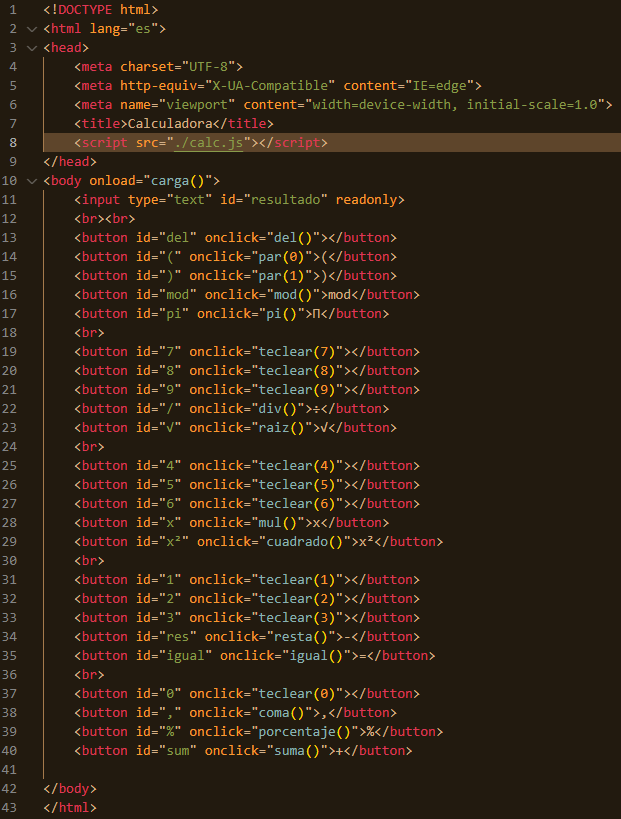
\includegraphics[width=0.8\textwidth,keepaspectratio]{src/e1/calc01.png}
	\end{figure}
	\begin{itemize}	
		\item El código JS hace que los botones se impriman en un orden correcto
	\end{itemize}
	\lstinputlisting[language=JavaScript, caption={Codigo Js para imprimir botones},numbers=left,]{src/e1/script01.js}
	\begin{figure}[H]
		\centering
		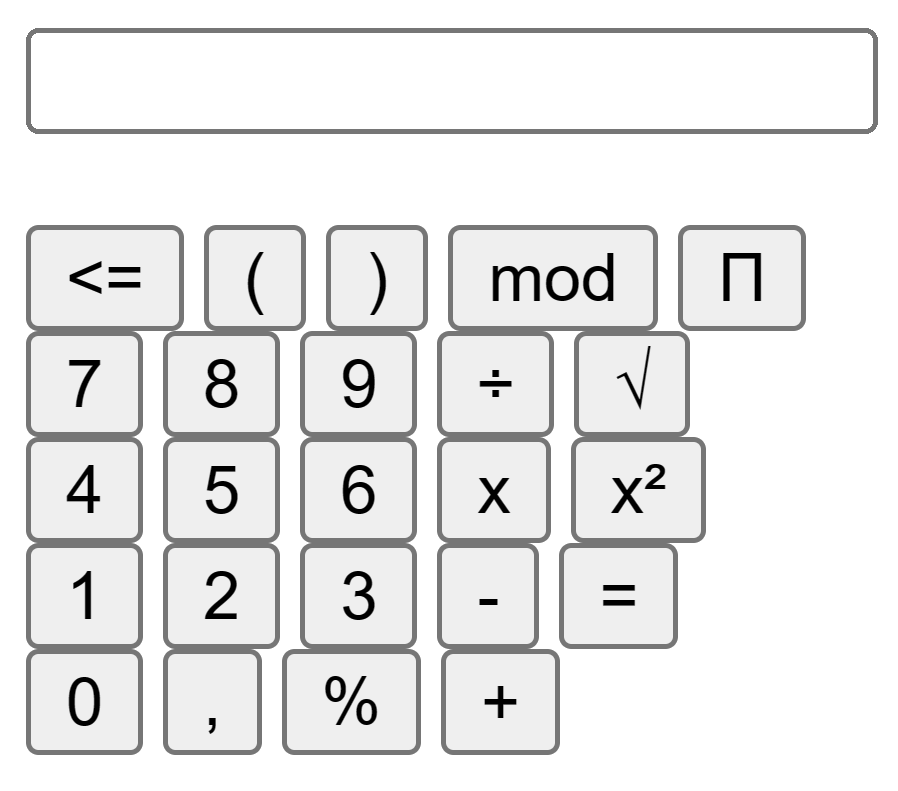
\includegraphics[width=0.3\textwidth,keepaspectratio]{img/calc01.png}
	\end{figure}
%%%%%%%%%%%%%%%%%%%%%%%%%%%%%%%%%%%%%%%%%%%%%%%%%%%%%
\subsection{Teclado con botones funcionales}
	\begin{itemize}	
		\item Cambiaron algunos nombres de las funciones para que se hiciera mas fácil de comprender
	\end{itemize}
	\begin{figure}[H]
		\centering
		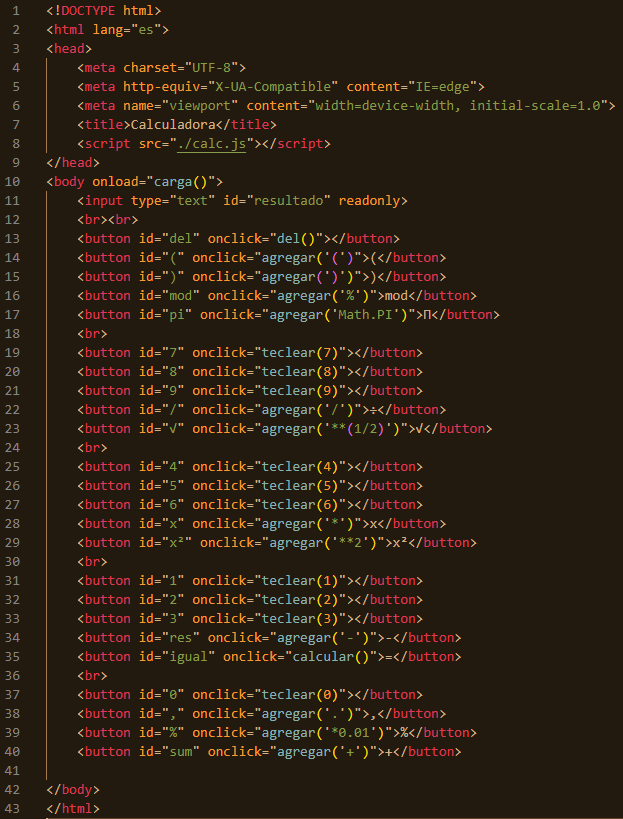
\includegraphics[width=0.8\textwidth,keepaspectratio]{src/e1/calc02.png}
	\end{figure}
	\begin{itemize}	
		\item Con la función eval de JavaScript se evalúa la función de la caja de texto
		que muestra como resultado la expresión como 5*5=25
	\end{itemize}
	\lstinputlisting[language=JavaScript, caption={Codigo JavaScript},numbers=left,]{src/e2/script02.js}
	\begin{figure}[H]
		\centering
		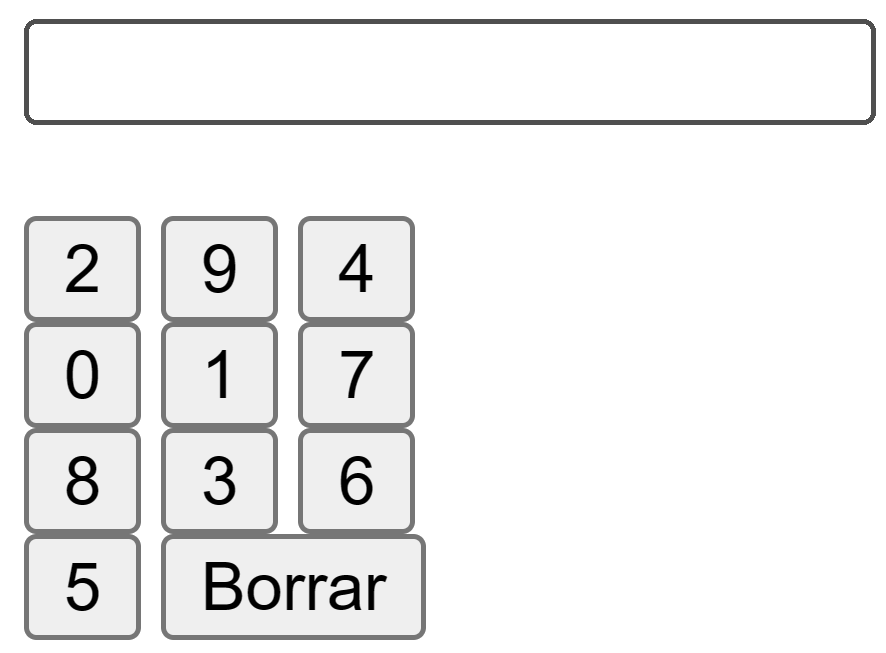
\includegraphics[width=0.5\textwidth,keepaspectratio]{img/calc02.png}
	\end{figure}
	\begin{figure}[H]
		\centering
		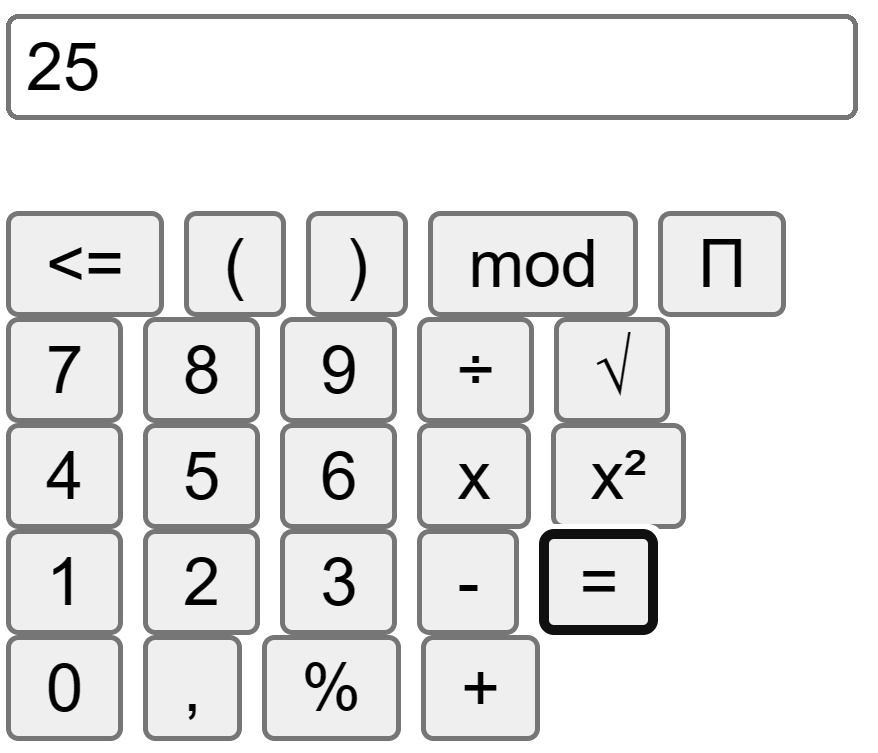
\includegraphics[width=0.5\textwidth,keepaspectratio]{img/calc03.png}
	\end{figure}
%%%%%%%%%%%%%%%%%%%%%%%%%%%%%%%%%%%%%%%%%%%%%%%%%%%%%
\subsection{Teclado con función de memorias}
	\lstinputlisting[language=HTMl, caption={Se implmento la función borrar},numbers=left,]{src/e2/index03.html}
	\begin{itemize}	
		\item Para borrar se dejaba en blanco el cuadro de texto
	\end{itemize}
	\lstinputlisting[language=JavaScript, caption={Codigo JavaScript},numbers=left,]{src/e2/script03.js}
	\lstinputlisting[language=CSS, caption={Codigo CSS},numbers=left,]{src/e2/css01.css}
	\begin{figure}[H]
		\centering
		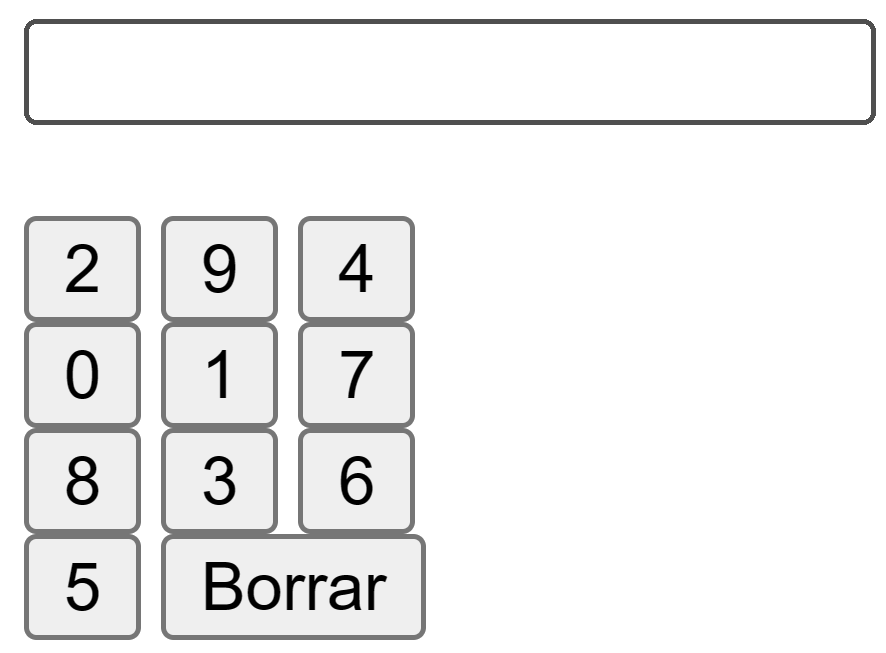
\includegraphics[width=0.3\textwidth,keepaspectratio]{img/tec02.png}
	\end{figure}
	\begin{figure}[H]
		\centering
		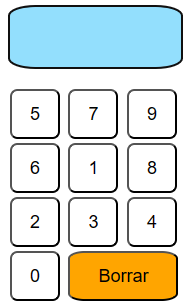
\includegraphics[width=0.3\textwidth,keepaspectratio]{img/tec03.png}
	\end{figure}
%%%%%%%%%%%%%%%%%%%%%%%%%%%%%%%%%%%%%%%%%%%%%%%%%%%%%
	%%%%%%%%%%%%%%%%%%%%%%%%%%%%%%%%%%%%%%%%%%%%%%%%%%%%%%%%%%%%
	%%%%%%%%%%%%%%%%%%%%%%%%%%%%%%%%%%%%%%%%%%%%%%%%%%%%%%%%%%%%
	\section{Ejercicio 2}
	\subsection{Implementación de teclado en orden con for de JS}
	\lstinputlisting[language=HTMl, caption={Index.html con divs para agregar los botones},numbers=left,]{src/e2/index01.html}
	\begin{itemize}	
		\item El código JS hace que los números se impriman en un orden relativamente correcto
	\end{itemize}
	\lstinputlisting[language=JavaScript, caption={Codigo JavaScript},numbers=left,]{src/e2/script01.js}
	\begin{figure}[H]
		\centering
		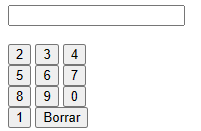
\includegraphics[width=0.3\textwidth,keepaspectratio]{img/tec01.png}
	\end{figure}
%%%%%%%%%%%%%%%%%%%%%%%%%%%%%%%%%%%%%%%%%%%%%%%%%%%%%
\subsection{Teclado desordenado con función JS}
	\lstinputlisting[language=HTMl, caption={Ahora los divs tienen su respectiva función},numbers=left,]{src/e2/index02.html}
	\begin{itemize}	
		\item En base al código brindado por Stackoverflow se creo la
		 función desorden que aleatoriza el teclado
	\end{itemize}
	\lstinputlisting[language=JavaScript, caption={Codigo JavaScript},numbers=left,]{src/e2/script02.js}
	\begin{figure}[H]
		\centering
		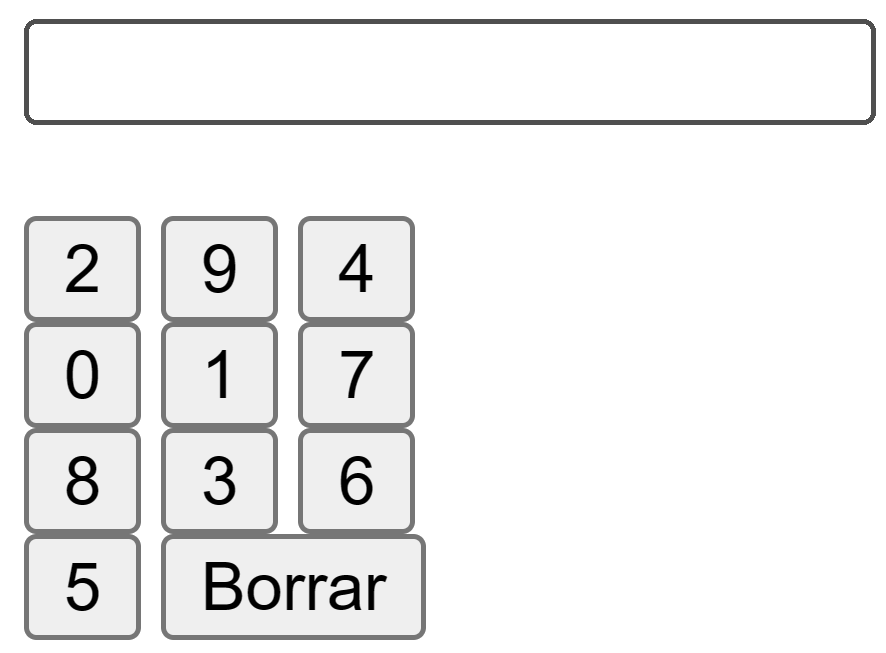
\includegraphics[width=0.3\textwidth,keepaspectratio]{img/tec02.png}
	\end{figure}
%%%%%%%%%%%%%%%%%%%%%%%%%%%%%%%%%%%%%%%%%%%%%%%%%%%%%
\subsection{Teclado terminado con borrado implementado}
	\lstinputlisting[language=HTMl, caption={Se implmento la función borrar},numbers=left,]{src/e2/index03.html}
	\begin{itemize}	
		\item Para borrar se dejaba en blanco el cuadro de texto
	\end{itemize}
	\lstinputlisting[language=JavaScript, caption={Codigo JavaScript},numbers=left,]{src/e2/script03.js}
	\lstinputlisting[language=CSS, caption={Codigo CSS},numbers=left,]{src/e2/css01.css}
	\begin{figure}[H]
		\centering
		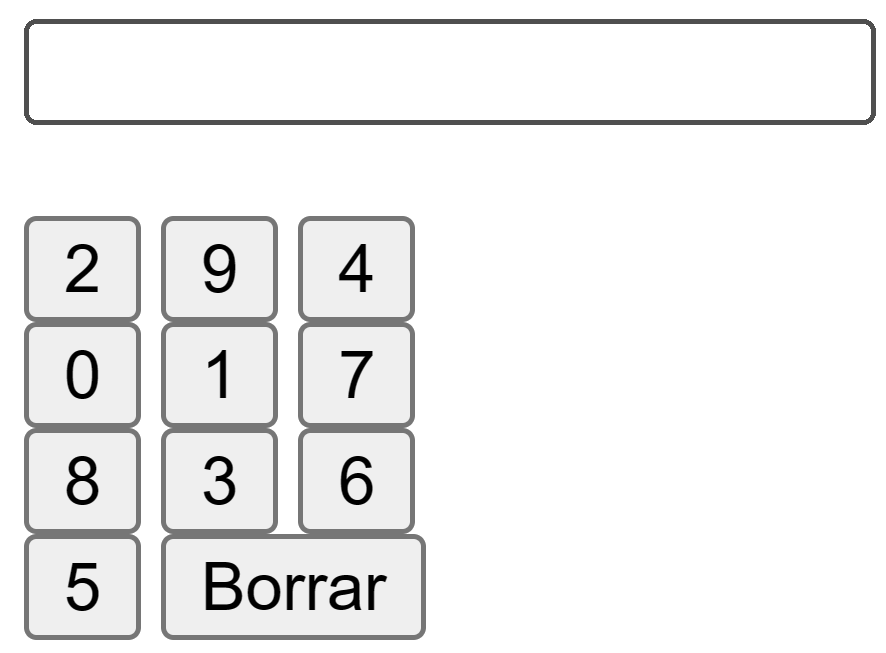
\includegraphics[width=0.3\textwidth,keepaspectratio]{img/tec02.png}
	\end{figure}
	\begin{figure}[H]
		\centering
		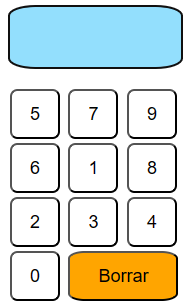
\includegraphics[width=0.3\textwidth,keepaspectratio]{img/tec03.png}
	\end{figure}
%%%%%%%%%%%%%%%%%%%%%%%%%%%%%%%%%%%%%%%%%%%%%%%%%%%%%
\begin{lstlisting}[style=ascii-tree]
	C:\USERS\PAULO\PW2-LAB-C-23A\LAB1
	|	estilos.css
	|	index.html
	|---fotos
	|		BusterYYo.jpg
	|---latex
		|	lab1_paulo-hidalgo.tex
		|   lab1_paulo-hidalgo.pdf
		|---build
		|		lab1_paulo-hidalgo.aux
		|       lab1_paulo-hidalgo.fdb_latexmk
		|       lab1_paulo-hidalgo.fls
		|       lab1_paulo-hidalgo.log
		|       lab1_paulo-hidalgo.out
		|       lab1_paulo-hidalgo.pdf
		|       lab1_paulo-hidalgo.synctex.gz
		|---img
		|		logo_abet.png
		|       logo_episunsa.png
		|       logo_unsa.jpg
		|       Segundo-commit.png
		|       ultimo-commit.png
		|---src
		|		css01.css
		|		index01.html
		|		index02.html
\end{lstlisting}    
	\clearpage
	\section{\textcolor{red}{Rúbrica para el contenido del Informe y demostración}}
	\begin{itemize}			
		\item El alumno debe marcar o dejar en blanco en celdas de la columna \textbf{Checklist} si cumplio con el ítem correspondiente.
		\item Si un alumno supera la fecha de entrega,  su calificación será sobre la nota mínima aprobada, siempre y cuando cumpla con todos lo items.
		\item El alumno debe autocalificarse en la columna \textbf{Estudiante} de acuerdo a la siguiente tabla:
	
		\begin{table}[ht]
			\caption{Niveles de desempeño}
			\begin{center}
			\begin{tabular}{ccccc}
    			\hline
    			 & \multicolumn{4}{c}{Nivel}\\
    			\cline{1-5}
    			\textbf{Puntos} & Insatisfactorio 25\%& En Proceso 50\% & Satisfactorio 75\% & Sobresaliente 100\%\\
    			\textbf{2.0}&0.5&1.0&1.5&2.0\\
    			\textbf{4.0}&1.0&2.0&3.0&4.0\\
    		\hline
			\end{tabular}
		\end{center}
	\end{table}	
	
	\end{itemize}
	
	\begin{table}[H]
		\caption{Rúbrica para contenido del Informe y demostración}
		\setlength{\tabcolsep}{0.5em} % for the horizontal padding
		{\renewcommand{\arraystretch}{1.5}% for the vertical padding
		%\begin{center}
		\begin{tabular}{|p{2.7cm}|p{7cm}|x{1.3cm}|p{1.2cm}|p{1.5cm}|p{1.1cm}|}
			\hline
    		\multicolumn{2}{|c|}{Contenido y demostración} & Puntos & Checklist & Estudiante & Profesor\\
			\hline
			\textbf{1. GitHub} & Hay enlace URL activo del directorio para el  laboratorio hacia su repositorio GitHub con código fuente terminado y fácil de revisar. &2 &X &2 & \\ 
			\hline
			\textbf{2. Commits} &  Hay capturas de pantalla de los commits más importantes con sus explicaciones detalladas. (El profesor puede preguntar para refrendar calificación). &4 &X &4 & \\ 
			\hline 
			\textbf{3. Código fuente} &  Hay porciones de código fuente importantes con numeración y explicaciones detalladas de sus funciones. &2 &X &2 & \\ 
			\hline 
			\textbf{4. Ejecución} & Se incluyen ejecuciones/pruebas del código fuente  explicadas gradualmente. &2 &X &2 & \\ 
			\hline			
			\textbf{5. Pregunta} & Se responde con completitud a la pregunta formulada en la tarea.  (El profesor puede preguntar para refrendar calificación).  &2 &X &2 & \\ 
			\hline	
			\textbf{6. Fechas} & Las fechas de modificación del código fuente estan dentro de los plazos de fecha de entrega establecidos. &2 &X &2 & \\ 
			\hline 
			\textbf{7. Ortografía} & El documento no muestra errores ortográficos. &2 &X &2 & \\ 
			\hline 
			\textbf{8. Madurez} & El Informe muestra de manera general una evolución de la madurez del código fuente,  explicaciones puntuales pero precisas y un acabado impecable.   (El profesor puede preguntar para refrendar calificación).  &4 &X &4 & \\ 
			\hline
			\multicolumn{2}{|c|}{\textbf{Total}} &20 & &20 & \\ 
			\hline
		\end{tabular}
		%\end{center}
		%\label{tab:multicol}
		}
	\end{table}
	
\clearpage

\section{Referencias}
\begin{itemize}			
	\item \url{https://www.w3.org/Style/Examples/011/firstcss.es.html}
\end{itemize}				
\end{document}